\section{Dataset}

\begin{frame}{About Dataset}
\begin{itemize}
    \item The Breast Cancer Wisconsin (Diagnostic) Data Set
    \item 569 rows with 33 attributes
    \item Features are computed from a digitized image of a fine needle aspirate (FNA) of a breast mass.
    \item Describe characteristics of the cell nuclei present in the image
\end{itemize}
  
\end{frame}

\begin{frame}{Parameter of Interest}
\begin{itemize}
    \item perimeter\_mean
    \item the mean size of the core tumor
    \vspace{0.25in}
    \begin{figure}
        \centering
        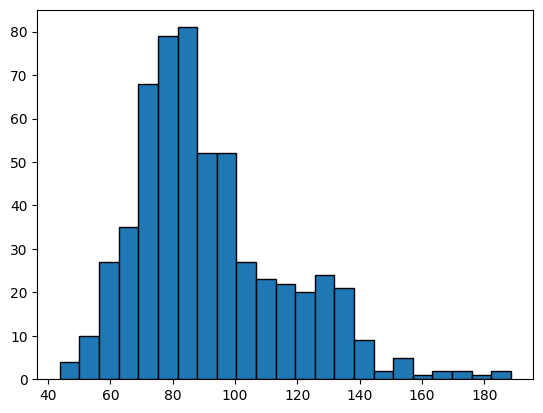
\includegraphics[width=0.5\linewidth]{Project1/Report/images/data-hist.png}
        \caption{Histogram of Perimeter Mean}
        \label{fig:enter-label}
    \end{figure}
\end{itemize}
  
\end{frame}

\section{Data Modelling}

\begin{frame}{Data Modelling}
\begin{itemize}
    \item Data looks like Skewed bell curved
    \item Modelled using Normal Distribution
\end{itemize}
  
\end{frame}

\begin{frame}{Box-Cox Transformation}
\begin{itemize}
    \item Used box-cox transformation to reduce skewness
    \item (Write formula of box-cox and explain what lambda signify in that)
    \begin{figure}
        \centering
        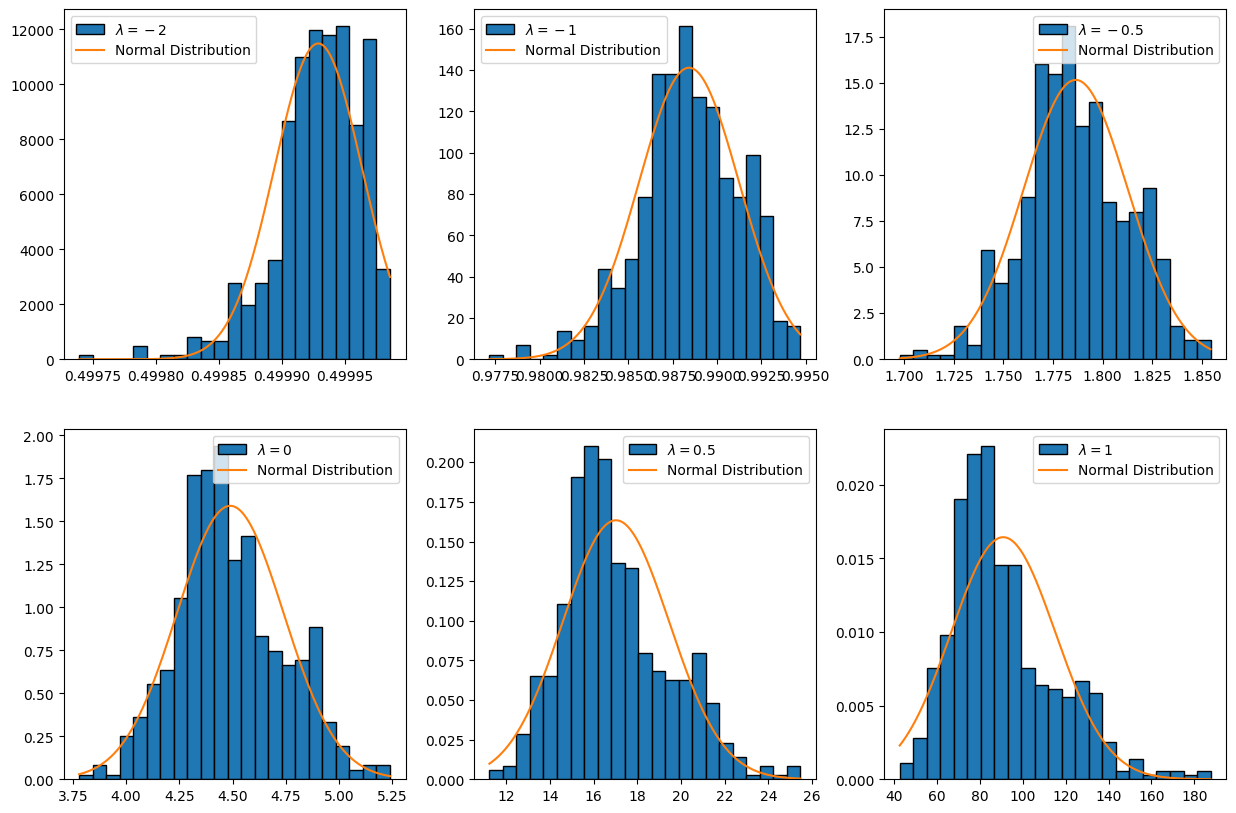
\includegraphics[width=0.5\linewidth]{Project1/Report/images/transforms.png}
        \caption{Transformation with different $\lambda$}
        \label{fig:enter-label}
    \end{figure}
\end{itemize}
  
\end{frame}
\begin{frame}{Box-Cox Transformation}
\begin{itemize}
    \item Used Q-Q (Quantile-Quantile) plots to visualize how well our transformation fits the normal distribution.
    \vspace{0.25in}
    \begin{figure}
        \centering
        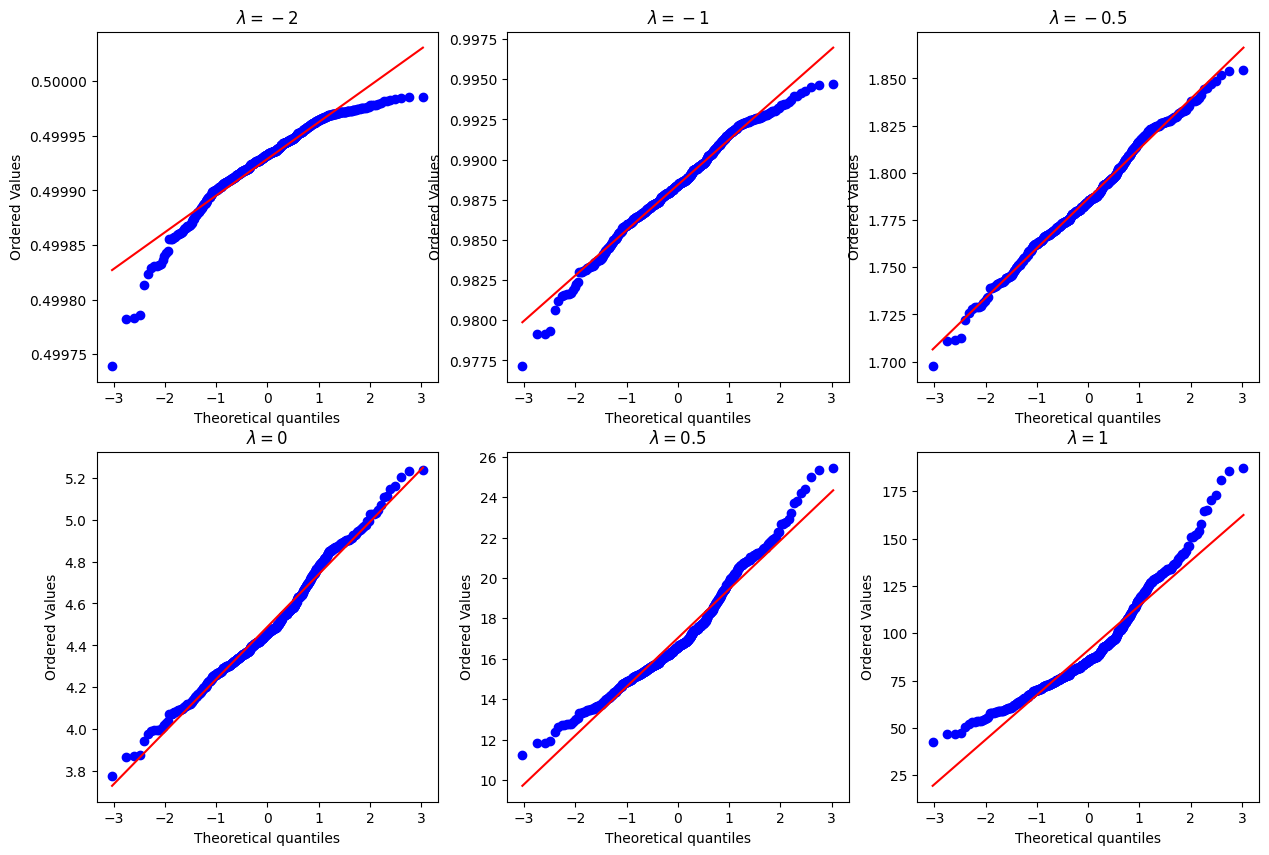
\includegraphics[width=0.5\linewidth]{Project1/Report/images/q-q.png}
        \caption{Q-Q Plot with different $\lambda$}
        \label{fig:enter-label}
    \end{figure}
\end{itemize}

\end{frame}

\begin{frame}{Finding Optimal Lambda for box-cox}
\begin{itemize}
    \item Normality of the transformation is calculated as the Pearson's correlation coefficient between the theoretical quantiles and the observed quantiles.
    \item (Write Formula of Pearson's correlation coefficient)
    \vspace{0.25in}
    \begin{figure}
        \centering
        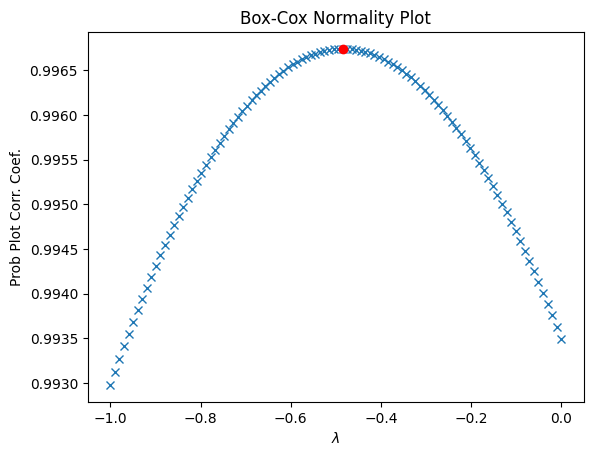
\includegraphics[width=0.5\linewidth]{Project1/Report/images/normality.png}
        \caption{Optimal $\lambda$}
        \label{fig:enter-label}
    \end{figure}
\end{itemize}
  
\end{frame}

\begin{frame}{Finding Optimal Lambda for box-cox}
\begin{itemize}
    \item \begin{figure}
        \centering
        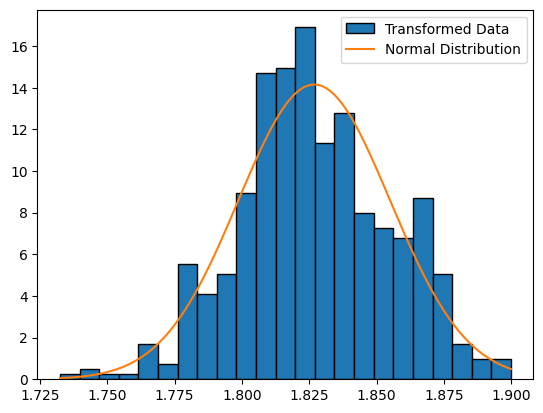
\includegraphics[width=0.5\linewidth]{Project1/Report/images/optimal-hist.png}
        \caption{Histogram of Data with Optimal $\lambda$}
        \label{fig:enter-label}
    \end{figure}
\end{itemize}
  
\end{frame}


\section{Bayesian Analysis of Model Parameters}

\begin{frame}{Bayesian Analysis of Mean}
\begin{itemize}
        \item (Show the mathematical calculation)
        \item (Some lines about prior)
        \item (Report prior, likelihood, posterior values)
        \begin{figure}
        \centering
        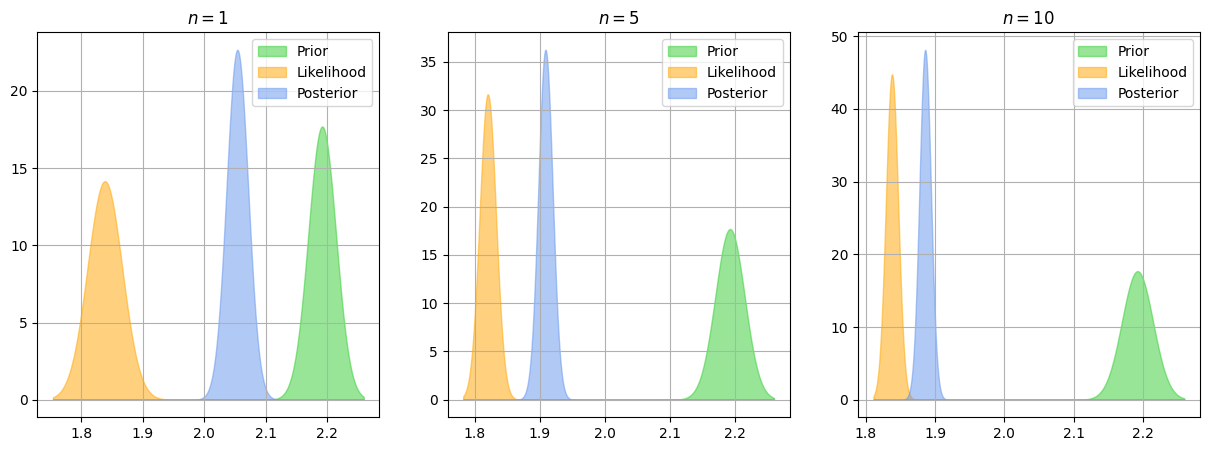
\includegraphics[width=0.5\linewidth]{Project1/Report/images/posterior.png}
        \caption{Posterior Analysis}
        \label{fig:enter-label}
    \end{figure}
\end{itemize}
  
\end{frame}

\begin{frame}{Central Posterior Interval}
\begin{itemize}
        \item (Show the mathematical calculation)
        \item (Report the value)
        \begin{figure}
        \centering
        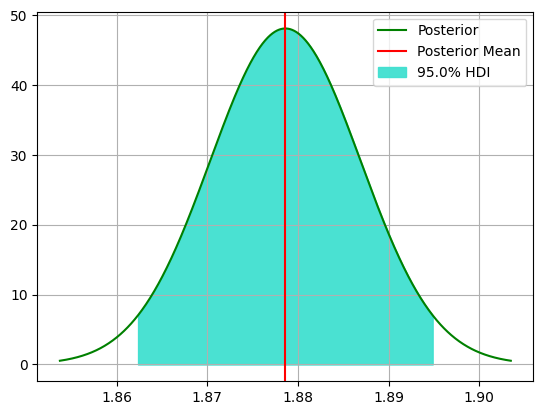
\includegraphics[width=0.5\linewidth]{Project1/Report/images/hdi.png}
        \caption{Central Posterior Interval}
        \label{fig:enter-label}
    \end{figure}
\end{itemize}
  
\end{frame}

\section{Inference/Conclusion}

\begin{frame}{Inference}
\begin{itemize}
        \item Line 1
        \item Line 2
        \item Line 3
\end{itemize}
  
\end{frame}
